\providecommand{\main}{..}
\documentclass[\main/tesi.tex]{subfiles}
\begin{document}
\chapter{Progettazione}

\section{Struttura della soluzione}
Il modulo è stato progettato con versatilità ed estensibilità in mente.\\
È infatti suddiviso in multipli \textbf{assembly}, ossia progetti .NET che vengono compilati in diverse \textbf{Dynamic Link Library}.\\

Tali assembly seguono un'architettura software a strati e sono, in ordine di dipendenze (ogni assembly riportato dipende da uno o più degli assembly riportati precedentemente):
\begin{itemize}
    \item \textbf{Dominio} (Micromed.Domain.Settings): Un assembly che contiene tutte le strutture di supporto (che saranno approfondite in seguito) utilizzate dal modulo.\\In particolare avremo le \textbf{entità}, ossia classi utilizzate come modelli di dominio da Entity Framework Core, nel quale ogni classe rappresenta una tabella.\\Altre classi degne di nota sono dei tipi generici che contengono il valore del settaggio, fornendo però altre informazioni relative alla centralizzazione.\\Si trovano in questo assembly anche vari \textbf{enum}, classi di supporto ed estensioni.
    \item \textbf{Astrazioni} (Micromed.Services.Settings.Abstractions): Si tratta dell'assembly più importante dal punto di vista della progettazione.\\Contiene infatti tutte le interfacce che il consumatore del modulo andrà ad utilizzare, senza necessità di conoscerne l'implementazione.\\Questo permette il \textbf{loose coupling} e una grande modularizzazione.
    \item \textbf{Persistenza} (Micromed.Data.Settings): L'assembly dedicato all'interfacciamento con i database (sia centrale che locale).\\Per evitare frammentazioni e inconsistenze, si utilizza la stessa sottoclasse di \textbf{DbContext} sia per il database locale che per quello remoto, creando istanze diverse con diverse \textbf{Connection String}.\\Contiene inoltre le implementazioni dei serializzatori che convertono oggetti complessi in stringhe salvabili a database (e viceversa).
    \item \textbf{Servizi} (Micromed.Services.Settings): Il centro del progetto, contiene l'implementazione del \textbf{SettingsService} e del servizio di configurazione.\\A livello operativo, l'utilizzatore andrà ad utilizzare (attraverso le apposite interfacce accennate precedentemente) sempre questi servizi, che saranno registrati tra i servizi sotto forma di \textit{singleton}.
    \item \textbf{Servizi di sincronizzazione} (Micromed.Services.Settings.Sync): Un assembly molto specifico, cotniene l'implementazione del \textbf{SettingsSyncService}, un servizio ausiliaro utilizzato dal principale SettingsService.\\Contiene tutte le logiche della sincronizzazione tra i database ed è stato progettato per avere un'interfaccia similme ad un servizio \textbf{REST}, prevedendo in futuro una diversa implementazione basata su richieste REST invece che su connessione diretta al database remoto.\\Anche per questo motivo è stato separato dal servizio principale, per essere intercambiabile.
    \item \textbf{Servizi Server} (Micromed.Services.Settings.Server): Assembly destinato ad uso esclusivo di programmi esterni a BrainQuick e FileManager contente un servizio con il compito di inizializzare o gestire il database centrale.\\Il primo consumatore di questo modulo è il programma che si occuperà della gestione delle policy, contenute nello stesso database centrale.\\
Tutte le interfacce legate agli ultimi quattro assembly citati si trovano tra le astrazioni.
\end{itemize}

Tale suddivisione segue la logica della \textit{Clean Architecture}, un'architettura che differisce dalla più classica "a strati" per essere costuita attorno ai principi dell'Inversion of Control e dalla completa separazione dei componenti che possono esistere autonomamente.\\

\begin{figure}[h]
    \label{fig:image_clean}
    \caption{Un diagramma che illustra l'architettura "pulita".}
    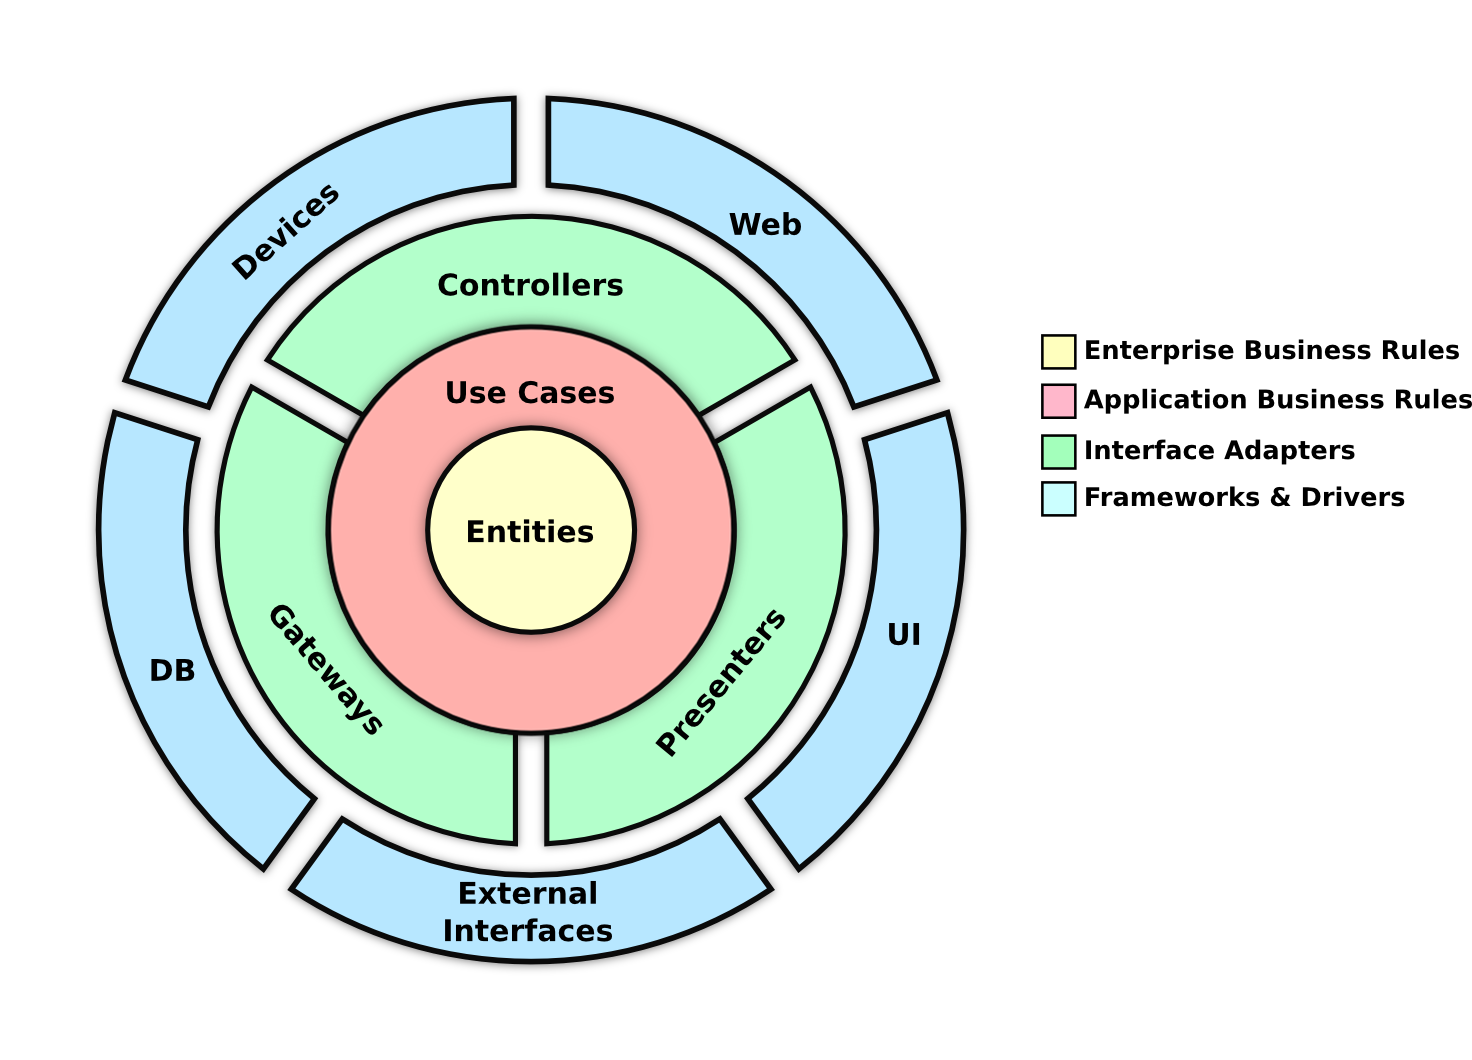
\includegraphics[width=\textwidth]{../images/clean.png}
\end{figure}

Questo ha permesso di costruire, sulla base delle astrazioni dedicate alla persistenza, due servizi differenti (SettingsService e SettingsServerService) completamente separati sia a livello di funzionalità che di assembly, oltre ad aver permesso di utilizzare i componenti minimi necessari per ciascun assembly dei software che devono implementare la soluzione.\\
Rispetto all'immagine \ref{fig:image_clean}, le astrazioni rappresentano i casi d'uso, il dominio rappresenta le entità mentre tutti i servizi (che sono indipendenti tra loro) sono contenuti nei blocchi più esterni.\\

\section{Strutture di supporto}
\label{strutturesupporto}
Data la complessità del modulo, i valori dei settaggi non possono essere utilizzati direttamente per questioni di sicurezza.\\
Infatti, data l'esistenza delle policy, non è detto che un settaggio sia modificabile, così come data la sincronizzazione, non è detto che un settaggio mantenga lo stesso valore nel tempo.\\
È necessario quindi utilizzare delle strutture di supporto, che forniscano azioni e funzionalità aggiuntive.\\
In particolare, ne sono presenti tre:
\begin{itemize}
    \item \textbf{Setting}: Una classe che rappresenta un singolo settaggio di uno dei tipi specificati nei requisiti.\\Nel caso si tratti di un vettore di valori, verrebbe trattato come un unico valore e di conseguenza qualsiasi modifica al vettore comporterebbe una totale riscrittura (ad esempio, nel caso due utenti aggiungessero due valori diversi in un settaggio rappresentato da un vettore, solo uno dei due verrebbe aggiunto sulla base delle politiche di sincronizzazione).
    \item \textbf{SettingSet}: Questa classe consiste in un insieme di settaggi, gestiti però separatamente.\\Consiste infatti in una collezione enumerabile ma non indicizzabile di SettingLeaf, ossia una variante di Setting
    \item \textbf{SettingLeaf}: Come accennato in precedenza, SettingLeaf non è altro che una classe molto simile a Setting, che aggiunge i riferimenti al \textit{parent} (ossia il SettingSet che lo contiene) e alcune proprietà che identificano in caso sia nuova (mai sincronizzata) o eliminata (quindi inutilizzabile solo localmente).
\end{itemize}
È notabile la differenza di gestione tra le prime due e la terza.\\
Mentre ogni istanza di Setting e SettingSet è unica rispettivamente al concetto alla quale è assegnata (e che quindi si comportano similmente ad singleton unico la cui unicità è relativa al concetto), le istanze di SettingLeaf hanno un lifetime legato alla loro esistenza nel sistema.\\
Essendo un numero variabile di figle di un SettingSet possono essere rimosse o aggiunte e la rimozione implica la loro eliminazione in quanto istanze.\\

Un'altra classe molto importante è \textbf{SettingsModel}, una classe astratta collegata al SettingService che fornisce dei metodi per ottenere le istanze dei vari settaggi.\\
Viene estesa dalle classi "contenitore" citate in precedenza che ne utilizzano i metodi e soprattutto, ne implementano un metodo astratto, chiamato \textbf{OnConfiguring}.\\
Questo metodo (la cui implementazione sarà discussa in seguito) viene richiamato dal SettingService per ogni istanza (singleton) delle classi contenitore che estendono SettingsModel per ottenere le informazioni necessarie a creare le istanze settaggi al primo avvio del software.

\section{Struttura del database}
La gestione del database segue un approccio \textbf{Code First} \cite{codefirst}, che consiste nel in non utilizzare direttamente gli strumenti forniti dal DBMS (ad esempio, file contenti script di query SQL) ma farlo indirettamente attraverso il livello di astrazione fornito da Entity Framework Core ed utilizzando il dominio dell'applicazione come linea guida per la creazione del database.\\
Di conseguenza, contrariamente ad un approccio \textbf{Database First}, il dominio di programma sarà la prima parte sviluppata e lo schema del database ne sarà subordinato.\\
Utilizzando la stessa logica, il database verrà creato ed inizializzato dal programma stesso al primo avvio, metodo che semplifica il lavoro dei tecnici che si occupano del \textit{deployment}.\\
La scelta di questo approccio è stata influenzata dall'utilizzo di EFCore, per il quale Microsoft stessa incoraggia l'approccio Code First.\\
Si sono inoltre considerati 
\begin{itemize}
    \item Una semplificazione in fase di sviluppo, in quanto la struttura e la gestione del database sono legate solamente al codice del software che andrà ad utilizzarlo, eliminando (per lo meno nel caso descritto) la necessità di script SQL accessori di cui tener conto.
    \item La semplificazione in fase di deployment, dato che la creazione e aggiornamento del database vengono automatizzati dal programma stesso (considerando la possibile presenza di centinaia di terminali da configurare).
    \item Una maggiore chiarezza e controllo, in quanto l'utilizzo di C\# invece di SQL fornisce alcuni vantaggi ad esempio sulla sintassi, che è uniforme anche per diversi DBMS a differenza delle implementazioni specifiche di SQL, oppure sulle relazioni delle tabelle, che vengono verificate a compile time.
\end{itemize} 
Per progetti precedenti è stato utilizzato l'approccio Database First, ma nel caso di un database piccolo e semplice come quello che sta venendo illustrato, l'approccio Code First è preferibile.\\

\begin{figure}[h]
    \caption{Lo schema ER del database}
    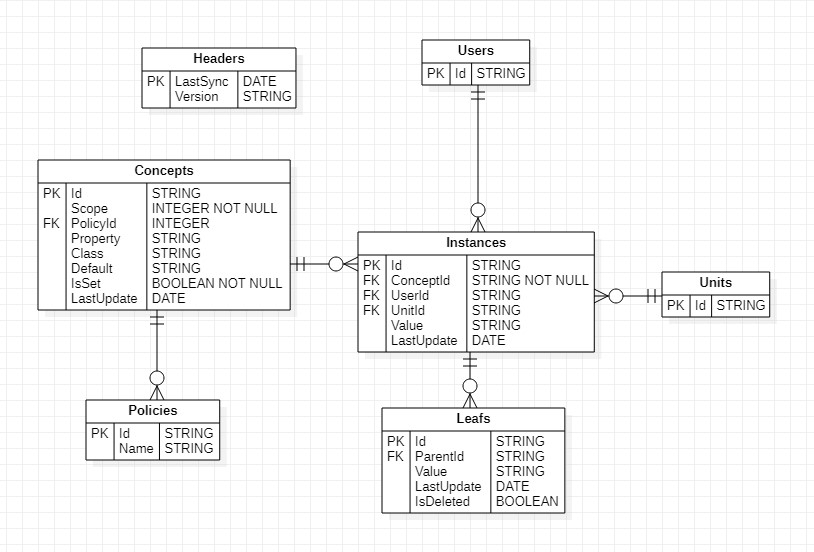
\includegraphics[width=\textwidth]{../images/er.png}
\end{figure}

Lo schema del database consiste in 7 tabelle:
\begin{itemize}
    \item \textbf{Concepts}: I record presenti in questa tabella identificano il \textit{concetto} associato a ciascun settaggio.\\Ogni concetto è un'entità unica, associata direttamente ad una proprietà nel codice che ne fornisce l'identificativo (un'UUID immutabile), il nome, la classe di appartenenza, lo scope ed opzionalmente il valore di default.
    \item \textbf{Instances}: Questa tabella contiene le \textit{istanze} relative ad un concetto.\\Similmente agli oggetti che nel mondo dellla programmazione sono realizzazioni di classi, nella soluzione che è stata progettata le istanze sono realizzazioni di un concetto relativamente a certe entità secondo lo scope del settaggio.\\Ad esempio, un'istanza di un settaggio con scope "UnitUser" sarà un record relazionato ad uno specifico concept, uno specifico utente e uno specifico terminale.\\Questa divisione tra concetti e istanze permette di mantenere i concetti immutati nel tempo, mantenendo quindi valori di default e policy intatte e non ridondate inutilmente.\\Le istanze contengono l'effettivo valore del settaggio e l'ultima data nella quale il valore è stato aggiornato.
    \item \textbf{Leafs}: Si tratta di una tabella molto simile a quella delle istanze, solo che al posto di contenere record relazionati ad un concept, le "foglie" sono relazionate ad un'istanza che non contiene valore (i valori sono infatti le foglie stesse).\\Inoltre, mentre una istanza una volta creata non può più essere rimossa, una foglia rappresenta un valore tra tanti collegati alla stessa istanza e può essere marcata come eliminata attraverso il campo "IsDeleted".
    \item \textbf{User}: Si tratta di una tabella contentente record ciascuno rappresentante un'utente.\\Di rilevante c'è solo l'identificativo, in quanto tutti gli altri dati sono contenuti in un altro database.
    \item \textbf{Unit}: Si tratta di una tabella contentente record ciascuno rappresentante una unità fisica nella quale è installato il software dell'azienda.\\Esattamente come la tabella Unit, contiene solamente l'identificativo.
    \item \textbf{Policies}: La tabella delle policy contiene tutte le informazioni relative alle varie policy definite dal cliente finale.\\In quanto la progettazione della gestione delle policy e del programma relativo è separata dal modulo dei settaggi centralizzati, lo schema della tabella è il più semplice possibile, contenente solo un campo per l'identificativo e uno per il nome della policy, mentre gli altri campi saranno definiti in una fase futura.
    \item \textbf{Headers}: Si tratta di una semplice tabella che contiene dei record che indicano la data dell'ultima sincronizzazione.\\Questi record sono essenziali per effettuare la sincronizzazione.
\end{itemize}

Come accennato in precedenza, le policy sono gestite separatamente rispetto al resto della soluzione, in quanto l'utilizzatore del modulo dei settaggi centralizzati non ha necessità di conoscere le policy collegate ad un determinato settaggio, che vengono applicate modificando direttamente le istanze contenute nel database centrale (con successiva sincronizzazione con i database locali).\\
In questo modo si è potuta sviluppare la soluzione in un periodo diverso rispetto alla gestione delle policy e quest'ultima può essere aggiornata senza influire sul resto del sistema.

\subsection{Serializzazione di strutture complesse}
\label{serialization}
Strutture complesse come i montaggi vengono serializzate nel formato JSON prima di essere salvate come stringhe nel database (sia esso locale o remoto).\\
Questo però introduce problemi di \textit{versioning}, in quanto modifiche alla struttura (come ad esempio l'aggiunta o la rimozione di un campo) potrebbero causare errori rispetto a dati salvati in precedenza.\\
È stato quindi deciso di applicare una serializzazione e deserializzazione custom, che inserisca (durante la deserializzazione) i campi sconosciuti all'interno di una mappa chiave-valore (resa accessibile ereditando la casse \textbf{SettingVersion}), in modo che non vengano persi (di default i serializzatori ignorano campi non riconosciuti) e vengano in seguito serializzati correttamente.
Nella sezione \ref{serializationimplementation} sarà discusso come sono state utilizzate alcune funzionalità di C\# per implementare questa soluzione.

\section{Configurazione}

Per ciascun programma distribuito in ciascun terminale appartenente al cliente finale verrà creato e compilato, dai tecnici che si occupano dell'installazione, un file JSON di configurazione che contiene le informazioni di connessione ed autenticazione (opportunamente criptate) ai rispettivi database, oltre ad alcune informazioni relative ad esempio al servizio di sincronizzazione automatica.\\
Non è previsto che i programmi modifichino il contenuto dei file in fase di esecuzione.\\
Questa configurazione verrà poi utilizzata da uno dei servizi che saranno descritti nella prossima sezione.\\

\subsection{I Servizi}
La configurazione del sistema di settaggi centralizzati comincia con la registrazione di tutti i servizi necessari al funzionamento nel \textit{Container} che gestisce le Dependency Injection.\\
I servizi richiesti sono diversi tra gli applicativi client che andranno ad utilizzare la centralizzazione dei settaggi e gli applicativi che andranno a configurare il database centrale.\\

\begin{figure}[h]
    \caption{La visualizzazione dei componenti della soluzione.}
    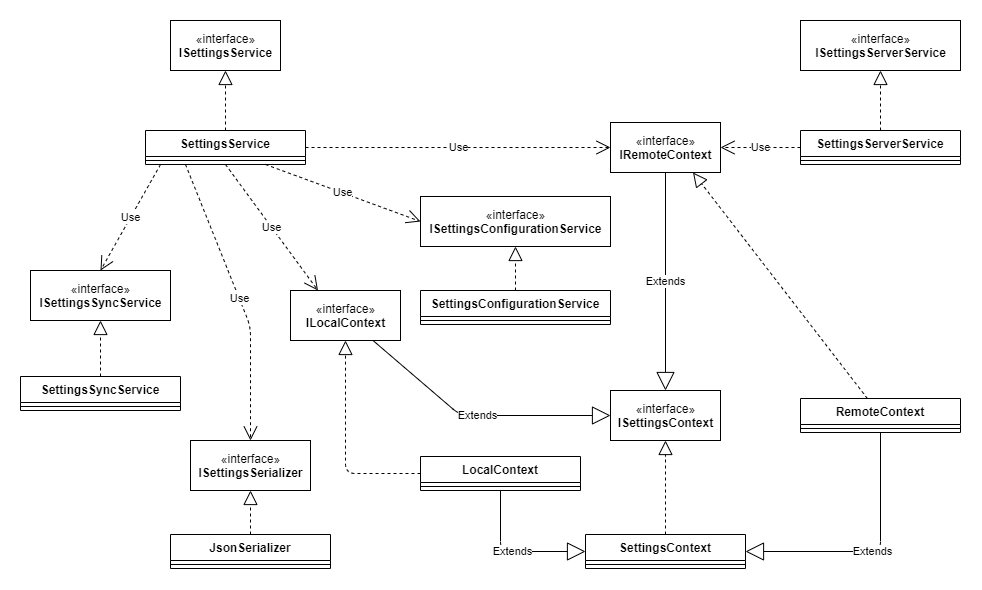
\includegraphics[width=\textwidth]{../images/components.png}
\end{figure}

In particolare i client necessiteranno di:
\begin{itemize}
    \item Il servizio che legge la configurazione JSON.
    \item Il servizio che genera le connessioni ai database.
    \item Il servizio di sincronizzazione.
    \item Il servizio di serializzazione.
\end{itemize}
Gli applicativi che si occuperanno della configurazione del database centrale differiscono per l'uso di un'implementazione di \textbf{ISettingsServerService} al posto di ISettingsService, del non aver bisogno della connessione al database locale e per l'assenza del servizio di sincronizzazione.\\

\section{Il flusso di esecuzione}
Per assicurarsi che la soluzione sia flessibile e in grado di gestire gli errori come richiesto dai requisiti, il flusso di esecuzione è stato diviso in diverse fasi:
\begin{itemize}
    \item \textbf{Inizializzazione}: Questa fase viene eseguita per prima (solitamente all'avvio) e solo una volta durante l'esecuzione del software.\\Consiste nel creare (nel caso non esista) il database locale, inizializzarlo con i valori di default e successivamente provare ad effettuare una versione limitata della sincronizzazione (nel caso sia abilitata la centralizzazione).\\Si può considerare la fase nella quale viene registrata l'unità (nel caso non sia già stata registrata) e completata la quale vengono resi disponibili i settaggi con scope "System" e "Unit".\\Vengono inoltre registrate tutte le istanze singleton che conterranno i settaggi (che sono caricati singolarmente in modo \textbf{lazy}).\\Un eventuale errore durante questa fase comporta l'impossibilità di procedere con le altre.
    \item \textbf{Login}: Si tratta della fase successiva all'inizializzazione, che può essere effettuata più volte durante l'esecuzione del programma, in quanto un diverso utente potrebbe accedere con diverse credenziali mentre il programma è in esecuzione.\\Durante questa fase viene registrato l'utente nel caso non lo sia già (si ricorda che il database che contiene tutte le informazioni dell'utente viene gestito separatamente, nel database dedicato alla centralizzazione dei settaggi viene salvato solo l'identificativo) e vengono resi disponibili i settaggi con scope "User" e "UnitUser".\\Nel caso di un cambiamento di utente, i settaggi relativi al precedente utente vengono eliminati dal database locale.\\In caso di errore durante questa fase parte dei settaggi non saranno disponibili.
    \item \textbf{Sync}: La fase di sincronizzazione completa può avvenire solo quando le due fasi precedenti (Inizializzazione e login) sono state portate a compimento senza errori.\\Può essere invocata multiple volte, sia manualmente da determinate azioni dell'utente sia in automatico dopo un certo intervallo di tempo.\\In caso di errore, qualsiasi modifica effettuata nei database fino a quel momento viene annullata, come approfondito nella sezione \ref{transazioni}.\\È una fase che viene completamente omessa in caso l'utente scelga una configurazione che non preveda la centralizzazione.
    \item \textbf{Refresh}: Questa fase viene eseguita in seguito a ciascuna delle precedenti.\\Consiste nell'aggiornare i valori dei settaggi (e di conseguenza sollevare eventuali eventi registrati) utilizzando i nuovi valori ottenuti dal completamento della fase immediatamente precedente.\\Un errore durante questa fase vanificherebbe la fase che lo precede, viene quindi considerato un errore interno a quest'ultima.\\Come accennato in precedenza, i \textit{Setting} e \textit{SettingSet} sono stati progettati per essere dei singleton dei quali venga solo aggiornato lo stato, ossia il valore che contengono per i primi e le foglie alle quali sono collegati per i secondi.\\I SettingLeaf invece sono cancellati e ricreati ad ogni refresh nel caso abbiano subito modifiche.
\end{itemize}

\begin{figure}[h]
    \caption{Il flusso di esecuzione rappresentato con un diagramma di flusso.}
    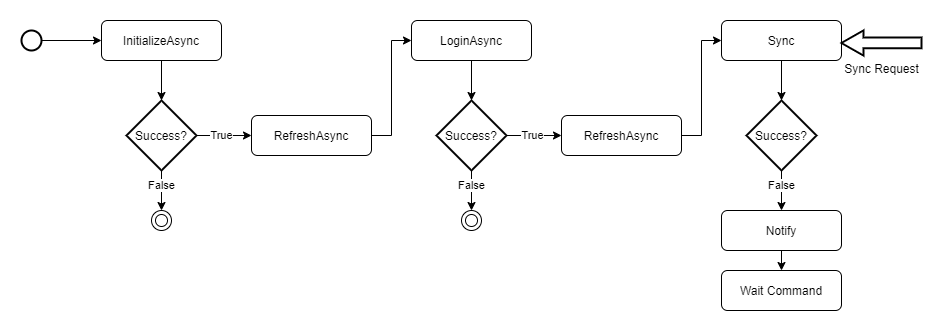
\includegraphics[width=\textwidth]{../images/execution.png}
\end{figure}

\subsection{La sincronizzazione}
La sincronizzazione è stata progettata per essere un assembly separato dal resto dei componenti del \textbf{SettingsService}, per facilitare l'integrazione di eventuali implementazioni alternative.\\
L'implementazione fornita di default riesce a soddisfare tutti i requisiti richiesti attraverso il SettingsSyncService, che effettua una \textit{fusione} delle diverse versioni dei settaggi, come indicato, attraverso un uso intensivo di Linq. 

\section{Il piano di integrazione}

L'integrazione di un modulo molto impattante a livello di funzionalità (si pensi ad esempio alle conseguenze che introduce la sincronizzazione automatica, dopo la quale il software deve adeguarsi alle modifiche nei valori dei settaggi) presenta la necessità di formulare una strategia che permetta una migrazione dal precedente sistema non centralizzato alla soluzione sviluppata introducendo il minor numero di problemi possibili.\\
È per questo che è stata effettuata un'analisi sul codice preeistente che ha portato ad un \textit{refactor} di alcune parti a forte utilizzo del sistema di settaggi precedente oltre ad ulteriori accorgimenti.

\subsection{Il refactor del codice esistente}
\label{refactor}
I due progetti che andranno ad utilizzare il modulo (come accenato in precedenza anch'essi in C\#) erano fermi ad una vecchia versione del .NET Framework non in grado di supportare la versione per cui sarebbe stata sviluppata la soluzione, ossia .NET Standard.\\
È stato quindi effettuato un upgrade alla versione 4.7 del runtime seguita dall'aggiornamento del formato dei file di configurazione dei progetti, risultando in una forte diminuzione del numero dei file di configurazione necessari (circa 100 tra i due progetti) oltre ad una maggiore compatibilità con .NET Core (verso il quale si prevede una migrazione in futuro).\\
Sono state inoltre isolate, ridotte e meglio documentate le porzioni di codice che necessitano dei settaggi, in previsione di una completa riscrittura.\\
In particolare la gestione dei \textit{montaggi} è stata progettata da zero in quanto il loro utilizzo influisce pesantemente sulle performance del software, di conseguenza la nuova implementazione (che aggiunge complessità) deve prevedere un minor numero di salvataggi.\\
È stato quindi deciso che il salvataggio dei montaggi sarebbe avvenuto solo su richiesta dell'utente attraverso l'interazione con una apposita UI.

\subsection{Pacchetti Nuget}
\label{nuget}
Come già accennato, la soluzione sviluppata deve essere integrata correntemente in due diversi progetti, i cui sorgenti risiedono in diversi \textit{stream}.\\
Inoltre è prevedibile che in futuro esistano l'azienda produca nuovi software che necessitano di una centralizzazione dei dati.\\
Per questi motivi si è scelto di sfruttare la flessibilità dei \textbf{pacchetti Nuget} per condividere il modulo tra i progetti utilizzando un server locale.\\
Per ogni assembly della soluzione viene creato un pacchetto che sarà poi installato negli assembly di BrainQuick e FileManager che lo richiedono.\\
Nuget gestisce automaticamente tutte le dipendenze e il fatto che ogni assembly sia un pacchetto diverso permette di installare nella maggior parte dei casi il solo pacchetto delle astrazioni, in quanto le effettive implementazioni saranno \textit{iniettate} usando le Dependency Injection.\\
Lo stesso procedimento si è poi utilizzato anche per altri assembly condivisi tra i due software che precedentemente venivano aggiornati sostituendo i file manualmente.

\subsection{Il testing}
Utilizzando la libreria xUnit per la scrittura di test automatici, sono stati implementati test unitari per multipli scenari, come ad esempio le fasi di inizializzazione e login, la sinronizzazione di tutti i tipi primitivi di settaggi (e con alcune classi per rappresentare oggetti complessi generici) e casi di conflitti durante la sincronizzazione.
Per semplificare i test è stata utilizzata un provider speciale di EFCore, chiamato \textbf{InMemory Database}, che simula un database in memoria volatile usa e getta.\\
Questa soluzione permette di evitare installazioni di database negli ambienti di testing, elimina la necessità di creare script di preparazione dei database e velocizza i tempi di esecuzione dei test.

\end{document}